\documentclass[sigconf]{acmart}

\usepackage{graphicx}
\usepackage{hyperref}
\usepackage{todonotes}

\usepackage{endfloat}
\renewcommand{\efloatseparator}{\mbox{}} % no new page between figures

\usepackage{booktabs} % For formal tables

\settopmatter{printacmref=false} % Removes citation information below abstract
\renewcommand\footnotetextcopyrightpermission[1]{} % removes footnote with conference information in first column
\pagestyle{plain} % removes running headers

\newcommand{\TODO}[1]{\todo[inline]{#1}}

\begin{document}

\title{Diagnosis of Coronary Artery Disease Using Big Data Analysis}
\author{Hady Sylla}
\orcid{HID339}
    \affiliation{%
    \institution{Indiana University}
    \streetaddress{711 N Park Ave}
    \city{Bloomington} 
    \state{Indiana} 
    \postcode{47408}
}
\email{hsylla@iu.edu}



\begin{abstract}
The Coronary artery disease (CAD) is the most prevalent heart complication. It is among the primary causes of worldwide heart failures and mortality \cite{ali}. Therefore, early diagnosis of this complication is essential. Specialists have invented different techniques for diagnosing CAD. They conduct most of these methods using the Irvine dataset (University of California), which have limitations of features and missing values thus unreliable. The study on the big data technique is seeking a latest set, with no missing values, consisting features like the Q wave, ST depression, functional class, T inversion, and dyspnea. The research compiled the data from the Shaheed Rajaei Cardiovascular, Medical and Research Center, between 2011 and 2012. The dataset include three features; Naïve Bayes, three hundred and three patients and SMO, and a proposed ensemble algorithm. The study uses the features to conduct the analyses. The researchers use the tenfold cross-validation to calculate accurate algorithms on the dataset by using the ensemble algorithm they present, and were eighty-eight point five accurate. Finally, the study extracts relevant features and rules regarding CAD, which previous studies did not discuss.

\end{abstract}

\keywords{i523, hid339, Coronary disease, big data, Random Forest}

\maketitle

\section{Introduction}
The CAD comes about when atherosclerotic plaques develop in the coronary arteries giving rise to the narrowing of coronary luminal, and sometimes, occlusion, which leads to heart failure or a sudden cardiac failure. In western nations, CAD is among the killer diseases. It is important for people to understand the CAD"s pathophysiology, how to control its development, identifying and effective innovation of the cardiovascular risk elements, and how to diagnose and treat it in early stages, and its reversible stages. The experts consider big data mining technique as "gold standard" for diagnosing CAD, and it is common in use. However, big data mining is an expensive and invasion procedure that requires a high-level of technological experience and latest technology thus the medical experts cannot use it to screen many patients or treat them.  Due to this, many health facilities utilize other noninvasive tools to diagnose CAD. The most popular of these methods are stress echocardiography (ECHO), electrocardiogram (ECG), and scintigraphy or SPECT. Additionally, the clinical setups currently use the coronary magnetic resonance angiography (CMRA) MSCT or EBCT. The objective of this study is showing how using big data mining technique to diagnose the Coronary Artery Disease is the best way to control heart attacks and deaths. The review discusses the features in the big data mining tool, how they derive the results, and discussion of the results. Additionally, the paper gives way to future studies and offers recommendations to improve the CAD complication field. 
\par Data mining is a technique of finding hidden information in a database. Nowadays, several fields use data mining as it has different applications like scientific discoveries, in entrepreneurship, and fraud detention. Data mining calculations work on databases, in which each information archive has several attributes.  One of these qualities is the class label, which discovers the data category. The data mining algorithms people use in problems solving are association rule mining, classification, regression analysis and clustering.
To classify algorithms, a researcher requires a learning phase on a labelled data set, which makes him/her decide on the missing test record class label. In the learning phase, a scientist constructs a classification model to predict the data label class label using its values features. Specialist categorises heart complications as cardiovascular and cardiomyopathy disorders. The Coronary Artery Disease (CAD) is a major cardiomyopathy complication subgroup which causes disability, serious illness, and even death as the disease affect oxygen and blood supply to the heart muscles. The early symptoms of heart disease comprise pain in the centre of the chest or a sense of numbness, and palpitation. Other signs are fainting fits or dizzy spells, and dyspnea on exertion. 
Due to the important nature of heart failures, it is essential to find out its causes. Currently, the primary goal of many scientific pursue is making an accurate diagnosis of cardiac complications. The researchers collect a great deal of information while examining CAD patients, and by processing the data, they reveal how the main features of cardiac disorders relate (e.g. the amount of cholesterol, blood pressure, etc.) and these complications' occurrence probability. The next chapter discusses several research articles that discuss this topic and relate it to what this study's findings.

\section{Discussion}
In this section, the paper provides selected examples of the potential of big data arising from the variety, volume and value of the data people realize. Additionally, it shows how big data are contributing to scientific advance in cardiovascular medicine from discovery of underlying disease mechanisms, disease taxonomy, of treatment relevant sub-types of disease which underpin drug development, and precision medicine.

\section{Contribution of Big Data to Coronary Artery Disease}

\subsection{Discovery in genetic and big data}
Lee, Noh and Ryu \cite{lee2011ire1} discuss that it is challenging to provide deep mechanistic insight in large-scale big data mining resources given the limited availability of genetic information in sufficient depth. Bespoke, recallable investigator-led studies such as East London Genes & Health (ELGH) and the NIHR BioResource enable the coupling of big data mining with extreme genotypes and facilitate their in depth study using bespoke experimental protocols. Complete gene knockouts inform people about gene process. With the latest survey of three thousand, two hundred and twenty-two  British Pakistani heritage exome sequenced persons with parental relatedness that is high, discover one thousand, one hundred and eleven rare-variant homozygous most likely function loss (rhLOF) genotypes predict to disrupt (knockout) seven hundred and eighty-one genes \cite{wang2005framingham}.
\par Srinnivas \cite{srinivas2010analysis}, Rajkumar \cite{rajkumar2010diagnosis} stated that linking big data to the rhLOF genotypes do not associate with a doctor or prescription consultation rate, and no illness-related phenotypes in thirty-three of forty-two individuals with rhLOF genotypes in Mendelian recessive complexity genes. Phasing the genome sequencing of a healthy PRDM9 knockout woman, her controls and baby, show meiotic recombination sites localised from the hotspots with PRDM9 dependent, depicting PRDM9 redundancy in human beings. Genomic approaches to validating case definitions: across 1000 s of hospital ICD codes, reproduce associations from genome-wide association studies obtained one phenotype at a time.

\subsection{Discovery in larger scale epidemiology}
Big health record data can contribute to the discovery of new associations, which would be hard to generate from traditional consented cohorts without record linkage.  This is resolution across a range of risk factor levels and a range of different initial presentations of cardiovascular disease. The discovery of various associations in a cohort of >1m adults initially free from diagnosed cardiovascular disease using national structured linked electronic health records from the CALIBER resource, in which EHR phenotyping algorithms are created, validated and shared using a robust methodology \cite{wang2005framingham}.
Sideman \cite{sideman1985simulation}argued that the primary precision medicine necessity is estimating the present patient's state. The experts mainly analze complication temporal and correlations illness trajectories with focus on few complications or by use of large-scale techniques without time consideration. Researchers perform a discovery-driven study on temporal illness progression patterns using data from an electronic health registry covering the entire Denmark population. Using the whole illness spectrum, they create 14.9 years of record data on six million, two hundred thousand patients into one thousand one hundred and seventy-one critical trajectories.The experts identify the primary diagnoses like chronic obstructive pulmonary disease and gout obstructive pulmonary disease as the cause of the CAD progression across many of these paths thus it is more significance to diagnose earlier. Such data-driven approach analysis is useful for preventing and predicting future complexities of individual patients \cite{sideman1985simulation}.

\subsection{Discovery with deep phenotypic data}
Most cardiovascular diseases (including acute myocardial infarction) have syndromic descriptions and labels, which may span multiple underlying pathological disease processes. One approach to discovering mechanistically relevant disease types is to phenomenal disease \cite{sahaf2011comparing}. For example, in heart failure with preserved ejection fraction machine learning in 46 continuous clinical, laboratory, electrocardiographic, and echocardiographic findings define mutually exclusive groups, which relate to subsequent outcomes. The cardiac atlas project (of healthy and diseased hearts) is an example of large-scale collaborations on feature extraction in imaging using data sharing in standard formats Digital Imaging and Communications in Medicine (DICOM) of the pixel and non-pixel data. Personalization using physiological simulations71 for example for cardiac resynchronisation the study propose therapy. Unstructured free-text data in big data mining adds a further resolution for estimation of disease co-occurrence and stratification of a patient stratification, which people map to the biology frameworks of systems \cite{sahaf2011comparing}.

\subsection{Discovery with deep phenotypic data}
Most cardiovascular diseases (including acute myocardial infarction) have syndromic descriptions and labels, which may span multiple underlying pathological disease processes. One approach to discovering mechanistically relevant disease types is to phenomap disease \cite{rajkumar2010diagnosis}. For example, in heart failure with preserved ejection fraction machine learning on 46 continuous clinical, laboratory, electrocardiographic, and echocardiographic findings define mutually exclusive groups, which relate to subsequent outcomes. The cardiac atlas project (of normal and diseased hearts) is an example of large scale collaborations on feature extraction in imaging using data sharing in standard formats Digital Imaging and Communications in Medicine (DICOM) of pixel and non-pixel data. Personalization using physiological simulations for example for cardiac resynchronization therapy is proposed. Unstructured free-text data in big data mining adds further resolution for estimation of disease co-occurrence and stratification of a patient stratification, which people map to the biology frameworks of systems \cite{rajkumar2010diagnosis}

\subsection{Discovering and validating drug targets}
Regarding a discussion by \cite{rajkumar2010diagnosis}, big data-DNA resources may play an increasingly important role in drug discovery, genomic drug target validation, and marker validation and drug repurposing. For example, demonstrates the strategy that human mutations that inactivate a gene encoding a drug target can mimic the action of an inhibitory drug, here ezetimibe, and thus can be used to infer potential effects of that drug \cite{rajkumar2010diagnosis}.  Ezetimibe is known to affect the marker (LDL cholesterol) but, until recently, not the disease (myocardial infarction). 
Among the most significant sources of cases of MI and controls in this study was a DNA resource integrated into a health system with rich big data.The discovery of PCSK9 as a drug target to lower cholesterol,79 which the EHR-DNA resources make in principle, illustrates the importance of rare variants in the identification of pathways relevant to the whole population. Mendelian randomisation studies are essential in evaluating whether markers such as heart rate and HDL cholesterol are causal for the disease of interest. Such genetic studies have questioned the role of heart rate and HDL cholesterol82 in the aetiology of heart attack \citep{palaniappan2008intelligent}.

\subsection{Cost effectiveness of innovation}
The Institute of Medicine (U.S.), Institute of Medicine (U.S.), and Institute of Medicine (U.S.) (2011) shows that big data provide new opportunities in understanding the cost-effectiveness of existing and new interventions. Because of the ability to assess baseline risks in unselected general populations (commonly higher risk than those reported in trials), such ‘real world evidence' is increasingly required by payers and the regulators. As more data sources are linked, greater granularity of the care data (e.g. 67 different types of primary care ‘consultation') may provide more accurate and more complete resource use data. For example, cost-effectiveness decision models can be developed before trials report to estimate the willingness to pay and pricing of a drug according to different trial benefits (relative risk reductions) applied to patients at various strata of risk \cite{muenke2015congenital}.

\subsection{Public health}
Agrawal \cite{agrawal1993mining} assert that there are significant gaps in our ability to prevent the onset of and prolong life in, many of the most common cardiovascular diseases in the 21st century including a trial fibrillation, heart failure, peripheral arterial disease. There are also gaps in our ability to measure disease and model the impact of interventions in populations. Clinicians diagnose more specific entities than ‘heart attack', ‘CHD' or ‘CVD' yet conventional consented cohorts have lacked the statistical size or the phenotypic resolution to measure clinically relevant sub-types of disease \cite{chu2009bayesian}. Big data can study the conditions that clinicians diagnose to provide scalable, population-based, updatable measurements of new disease burden vital for the evaluation of alternative strategies of prevention. For example, significant data can be used to estimate the incidence and survival of the treatment-relevant sub-types of MI (ST elevation and non-ST elevation) \cite{dietterich2000ensemble}.

\section{Analysis}
To characterize algorithms, a researcher requires a learning stage on a labelled dataset collection, which makes him/her settle on the missing test record class \cite{ali}. In the learning stage, a researcher builds an order model model to predict the data label class label using its values features. Specialist categorises heart complications as cardiovascular and cardiomyopathy disorders \cite{ali}. The Coronary Artery Disease (CAD) is a noteworthy cardiomyopathy inconvenience subgroup which causes inability, genuine sickness, and even death as the disease affect oxygen and blood supply to the heart muscles. The early indications of coronary illness involve torment in the focal point of the chest or a feeling of deadness, and palpitation. Different signs are blacking out fits or mixed up spells, and dyspnea on effort.
\par  Due to the vital idea of heart failure, the primary goal of many scientific pursue is making an accurate diagnosis of cardiac complications. The analysts gather a lot of data while looking at CAD patients, and by preparing the information, they uncover how the main features highlights of cardiovascular issue relate (e.g. the measure of cholesterol, circulatory strain, and so on.) and these complexities' event likelihood.

\subsection{Dataset}
A dataset, constructed from the information collected from 303  random  visitors  (216  patients)  to  Shaheed Rajaei Cardiovascular,  Medical  and  Research  Center, was used to evaluate the effects of different demographic, clinical, and ECG features on the diagnosis of Coronary artery disease.This dataset is publicly available and does not contain any patient identifier.Demographics such as age and sex are also included in the dataset.

\subsection{Method}
I will use Random Forest machine learning for predicting the feature to diagnose coronary artery disease Random forests (RF) is a prominent tree-based ensemble machine learning tool that is exceptionally data adaptive \cite{breiman2001random}.I will primarily be using the SciPy stack, especially pandas, matplotlib, seaborn and sklearn.
I am using the describe() method that will give me basic statistics for every column in the dataset. This method will allow me to Generates descriptive statistics that summarize the central tendency, dispersion and shape of a dataset.

\begin{table}
\centering
\caption{Dastaset Description}
\label{my-label}
\begin{tabular}{llllllllllllllllllllll}
Age & Weight & Length & Sex & BMI   & DM        & HTN & Current Smoker & EX-Smoker & FH & ... & K   & Na  & WBC & Lymph & Neut & PLT & EF-TTE & Region RWMA & VHD & Cath   &        \\
0   & 53     & 90     & 175 & Male  & 29.387755 & 0   & 1              & 1         & 0  & 0   & ... & 4.7 & 141 & 5700  & 39   & 52  & 261    & 50          & 0   & N      & Cad    \\
1   & 67     & 70     & 157 & Fmale & 28.398718 & 0   & 1              & 0         & 0  & 0   & ... & 4.7 & 156 & 7700  & 38   & 55  & 165    & 40          & 4   & N      & Cad    \\
2   & 54     & 54     & 164 & Male  & 20.077335 & 0   & 0              & 1         & 0  & 0   & ... & 4.7 & 139 & 7400  & 38   & 60  & 230    & 40          & 2   & mild   & Cad    \\
3   & 66     & 67     & 158 & Fmale & 26.838648 & 0   & 1              & 0         & 0  & 0   & ... & 4.4 & 142 & 13000 & 18   & 72  & 742    & 55          & 0   & Severe & Normal \\
4   & 50     & 87     & 153 & Fmale & 37.165193 & 0   & 1              & 0         & 0  & 0   & ... & 4.0 & 140 & 9200  & 55   & 39  & 274    & 50          & 0   & Severe & Normal
\end{tabular}
\end{table}



For a better visualization of the data, I will generate a histogram. data visualization facilitate how to interpret and break down big data in a manner that is easily understandable.
\begin{figure}
    \centering
    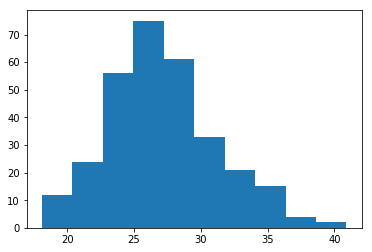
\includegraphics[width=1.0\columnwidth]{images/output_2_0.png}
    \caption{Bar Plot}
    \label{Plot}
\end{figure}



\subsection{Data Preparation}
Since this dataset include string data, I will use encoding to transforms categorical features to a format that works better with classification by taking all categorical features that have only 2 levels and label encoding them to get binary features. 

\begin{figure}
    \centering
    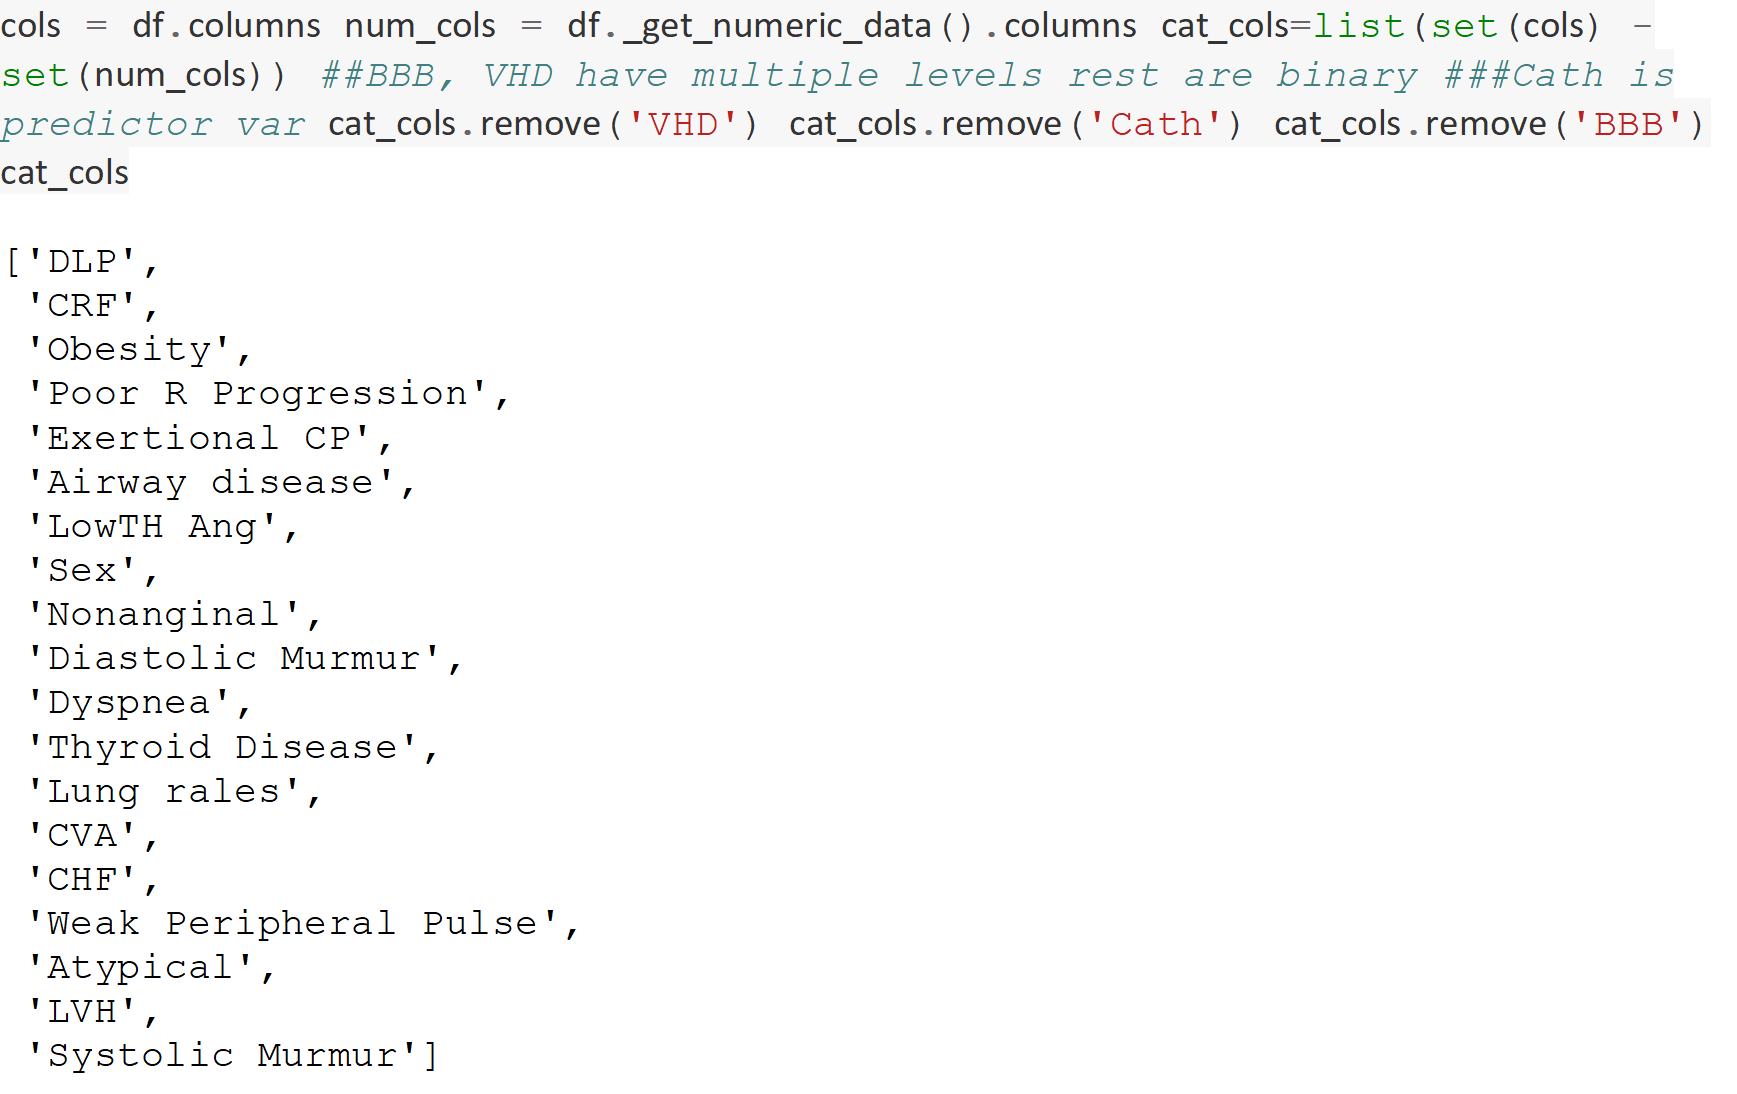
\includegraphics[width=1.0\columnwidth]{images/Untitled3.png}
    \caption{Encoding}
    \label{Encoding}
\end{figure}

Then I will apply one hot encoding our multiple level features that will allows the representation of categorical data to be more expressive.

\begin{figure}
    \centering
    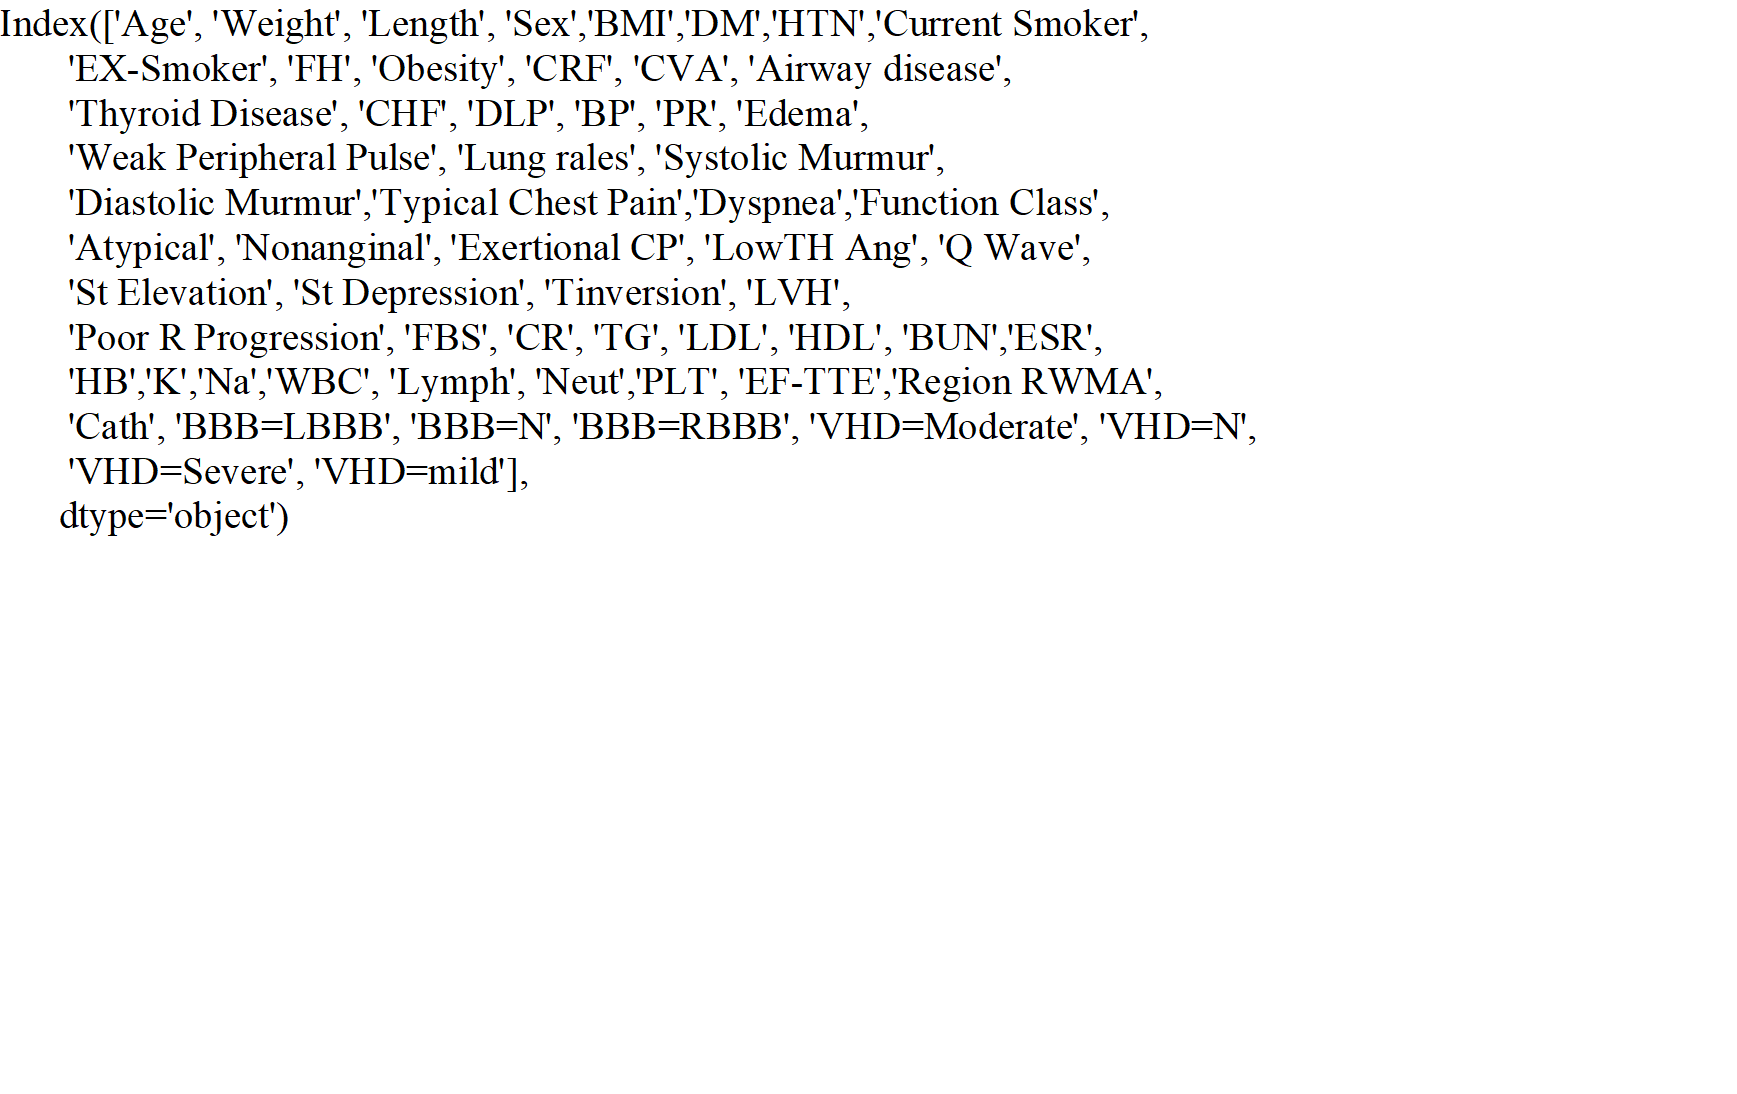
\includegraphics[width=1.0\columnwidth]{images/Encoding.png}
    \caption{Hot Encoding}
    \label{Hot Enco}
\end{figure}
    
\subsection{Measure of Variable importance Ranking}
An essential element of RF is that it gives a quickly calculable inner measure of variable significance (VIMP) that can be utilized to rank factors. This element is particularly valuable for high-dimensional genomic information.In spite of the fact that there are numerous fruitful applications utilizing change significance, a feedback is that it is a ranked based approach. Ranking is significantly more troublesome than the variable determination issue, which just tries to choose a gathering of factors that when consolidated are prescient, without forcing a positioning structure. In any case, in view of the many-sided quality in organic frameworks, positioned quality records in light of RF or RSF which consider relationship and communication impacts are as yet an immense change from univariate positioned quality records in light of t-test's or Cox corresponding peril demonstrating utilizing one variable at any given moment. Be that as it may, alert is required when deciphering any straight positioning since it is as a rule likely that various arrangements of feebly prescient highlights are mutually prescient. This seems, by all accounts, to be an uncertain issue of positioning and further investigations are required.
I will specify which dataset and variable I want to predict respectively.I like to keep a parameter file where I specify data sources and such. This lets me create generic analytics code that is easy to reuse.
After I have specified what dataset I want to study, I split the training and test datasets. Then I will scale the data, which makes most classifiers run better.

\begin{figure}
    \centering
    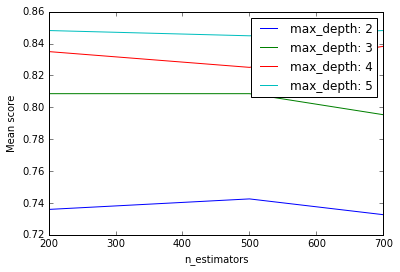
\includegraphics[width=1.0\columnwidth]{images/output_15_1.png}
    \caption{Scores Attribute}
    \label{Score}
\end{figure}

\begin{figure}
    \centering
    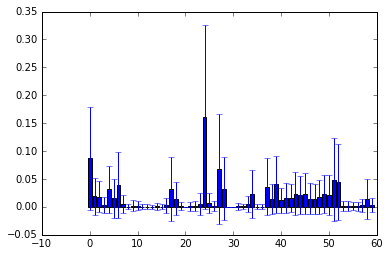
\includegraphics[width=1.0\columnwidth]{images/output_17_0.png}
    \caption{feature importance with their standard deviations}
    \label{Featites Format}
\end{figure}

\begin{table}
\centering
\caption{Feature Importance Table}
\label{Importance}
\begin{tabular}{lll}
Importance            & Std      &          \\
Age                   & 0.086779 & 0.092552 \\
Weight                & 0.018672 & 0.032956 \\
Length                & 0.018183 & 0.027928 \\
Sex                   & 0.003414 & 0.013603 \\
BMI                   & 0.031609 & 0.042215 \\
DM                    & 0.015427 & 0.034442 \\
HTN                   & 0.038735 & 0.059296 \\
Current Smoker        & 0.005287 & 0.015965 \\
EX-Smoker             & 0.000587 & 0.004463 \\
FH                    & 0.002472 & 0.010216 \\
Obesity               & 0.002333 & 0.008439 \\
CRF                   & 0.000534 & 0.004805 \\
CVA                   & 0.000469 & 0.004108 \\
Airway disease        & 0.000474 & 0.003385 \\
Thyroid Disease       & 0.001086 & 0.006045 \\
DLP                   & 0.000407 & 0.004046 \\
BP                    & 0.003296 & 0.013382 \\
PR                    & 0.031988 & 0.056958 \\
Edema                 & 0.014277 & 0.029568 \\
Weak Peripheral Pulse & 0.001758 & 0.007496 \\
Lung rales            & 0        & 0        \\
Systolic Murmur       & 0.001332 & 0.007931 \\
Diastolic Murmur      & 0.001853 & 0.008916 \\
Typical Chest Pain    & 0.00495  & 0.020264 \\
Dyspnea               & 0.161378 & 0.165277 \\
Function Class        & 0.006237 & 0.01781  \\
Atypical              & 0.001798 & 0.008412 \\
Nonanginal            & 0.067681 & 0.098911 \\
Exertional CP         & 0.032299 & 0.056285 \\
LowTH Ang             & 0        & 0        \\
Q Wave                & 0        & 0        \\
St Elevation          & 0.000976 & 0.005923 \\
St Depression         & 0.005336 & 0.014798
\end{tabular}
\end{table}
Finally by checking the model's accuracy on test set as shown on figure below, the accuracy score on test by Random Forest:0.8852.
\begin{figure}
    \centering
    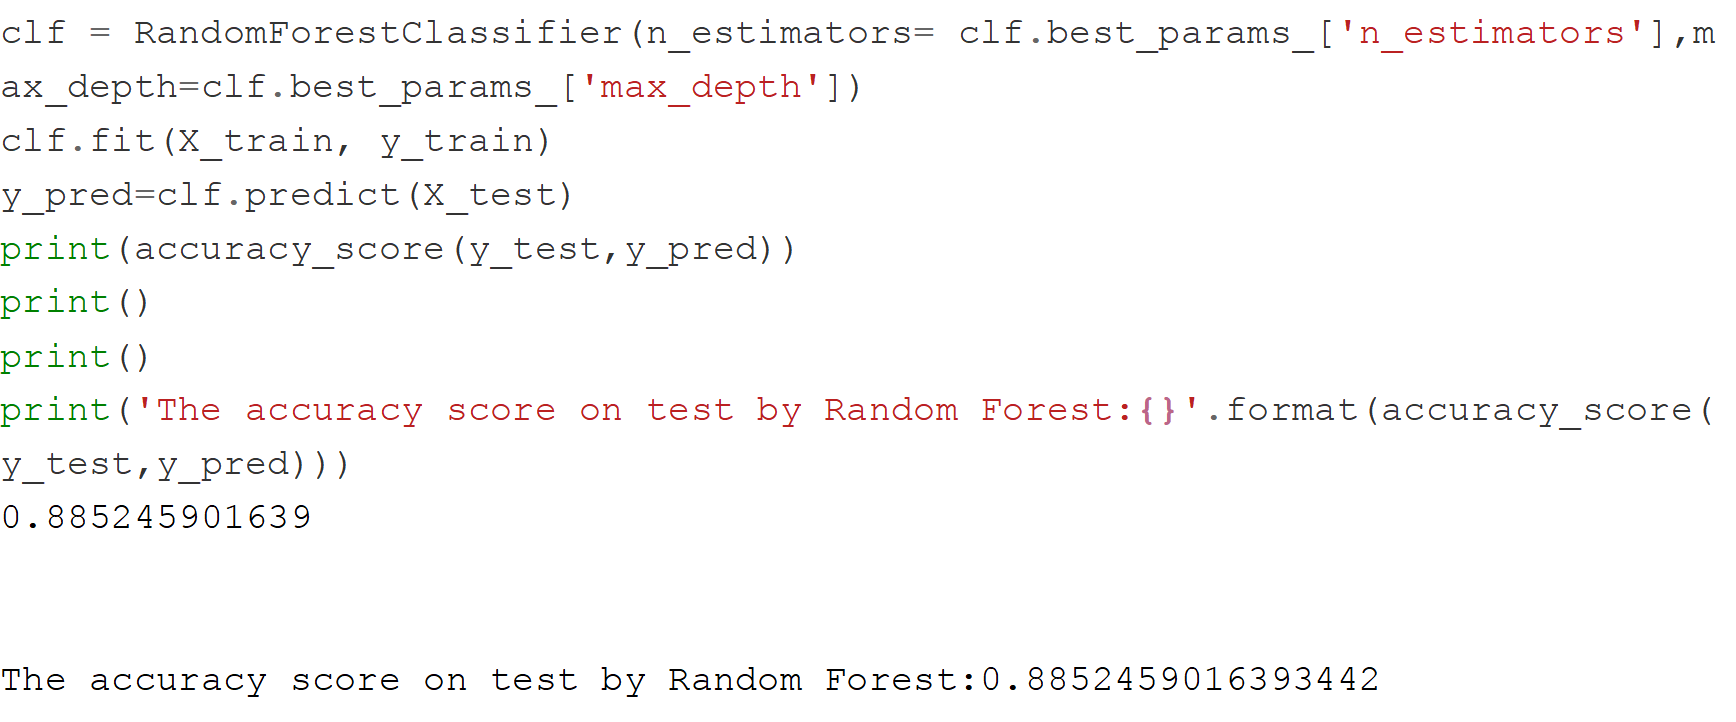
\includegraphics[width=1.0\columnwidth]{project/images/Untitled7.png}
    \caption{Accuracy Test}
    \label{Accuracy}
\end{figure}





\section{Conclusion}
The research uses a new dataset comprising thirty-eight features together with the data mining methods to get useful results about this area of research. Afterwards, the study chooses sixteen features using an element selection algorithm and some common classification algorithms, and it applies the ensemble algorithm it proposes on the dataset. The research obtains the highest accuracy (88.51%) when both the element selection and it uses the ensemble algorithm. Additionally, the study utilises the association rule mining methods to extract from the dataset the high confidential rules. The CAD complication is among the primary causes of deaths in the world. Thus people must put measures in place to predict, treat, and control the disease. The use of big data mining technique will help achieve this, therefore, reduce the mortality rate of people with the complexity. Additionally, not only the medical experts should know the use of this technique, but the entire community to save lives because the heart failures happen at unexpected times.
\par The objectives of the future studies should be adding other features like echo and lab echo data to investigate the effect of these elements on CAD diagnosis and get a higher accuracy in predicting the complication. Furthermore, the future works should utilise more algorithms and data mining techniques to improve the findings. Finally, the studies should extend the dataset with more sick people who can help in finding interesting results which may not be apparent for the patients the dataset it introduces. Another aim of the future research should be simplifying the use of big data mining method to make it user-friendly; this will make many medical facilities adopt the idea. Moreover, the future studies should research on other tools that can improve the big data mining technique's process thus making it less costly and require less technological know-how.

\section{Recommendations for Future Studies}
Many nations in the world have Big data mining systems that research can utilise hence to enable the research potential of these information sources; the countries have to centralise resources that govern the research dataset. Some states have initiatives towards achieving this although few tackle all elements of this procedure. For example, the CALIBER platform, which is in the United Kingdom, joints a repository of big data mining phenotypes with curates register linkages combining disease registry (Myocardial Ischaemia Nation Audit Project). Additionally, it joins primary care (Clinical Practice Research Datalink), death registry (Office of National Statistics), and hospital discharge (Hospital Episode Statistics) data in over two million adults with ten million individuals’ follow-up years. However, this resource does not offer tools for bidirectional relations with big data mining information sources. The United States National Human Genome Research Institute-funded consortium, the eMERGE Network, combines big data mining with a phenotype repository from multiple secondary healthcare systems, including text and imaging, joined to genotypic data for all candidates. Finally, the Clinical Record Interactive Search system, which is at the Maudsley NHS Foundation Trust, NIHR Mental Health Biomedical Research Centre and Dementia, and South London's Dementia Unit help researchers. The Clinical Record Interactive Search system allows scholars to analyse secondary data, comprising clinical notes and other texts, through simple tools that help to identify patients are attaining specific criteria and developing the text-mining algorithms.
\par Regarding this, the National big data mining portals can join the strengths of these projects by comprising: (i) Standards-driven types of equipment that enable reviewers to create interventional and observational studies. (ii) A countrywide catalogue of contemporary big data mining sources which is metadata standards curated. (iii)  Big data mining phenotype algorithms with an interactive thesaurus. By accomplishing this, the national catalogue can support the metadata integration and harvest from manual curation and external sources by researchers within a reproducible and standardised framework, and also offer guide people on data content and access. Due to this, users will identify information sources that provide data both across and within disease areas.
\par The big data mining dataset and algorithms creation equipment require implementation in a way that supports modification and reuse by other users, as well as the academic citation and credit that is appropriate. Creating this form of resource enables fostering an ‘open source' approach to big data mining research in which researchers learn and collaborate with one another. It eventually produces an advance in big data mining review than any other research group in isolation can achieve.


\begin{acks}
The authors would like to thank professor Gregor von Laszewski and his team assistance to provide me the tool and knowledge to complete this project.
\end{acks}

\bibliographystyle{ACM-Reference-Format}
\bibliography{report} 


\newpage
\appendix
\section{Code Reference}
All code and files for this project can be found in the githup repository:
\url{https://github.com/bigdata-i523/hid339/blob/master/project/code}

\end{document}
